\section{Implementation and Evaluation}\label{sec:experiment}

%Let's call sec 5 Implementation. In this sec, you first *briefly* talks about the implementation of the runtime system (in one subsec), and then you present the three examples with their respective GCC code. Then you present the eval results of these three examples with different scales (# of agents), etc. Finally you mention the web demo, and if possible show a snap shot of the web demo. I think that would be sufficient for this paper.

We have implemented a proof-of-concept system to show the viability of 
the speculative nondeterminism in a practical setting with typical
imperative languages.\footnote{A web demo of the system is
set up at \url{http://adapt.seiee.sjtu.edu.cn/speculate} and
all the code examples are included there.}
The implementation uses a client-server architecture with
a \emph{coordination server} written in 
Java, and a C library which provides speculation primitives.
The speculation primitives are embedded in an agent program
written using a imperative language, C or C++., and 
agent programs act as clients and communicate with the server 
via TCP connections.
The agents and coordination server form a distributed system.

We implement agents as Linux processes which can \emph{fork} 
into multiple processes if they create choices.
The coordination server maintains all runtime information of 
the universe, galaxies and worlds.
%In the environment of the agent, each process conceptually lives in 
%one or more worlds but still within one galaxy.
The system assumes a tuple space data model and uses data
operations similar to Linda, such as $in/out/rd$.

Next we describe a few optimizations that make the implementation
more practical, and then present three benchmark cases followed by
the evaluation of these benchmarks.

\subsection{Optimizations}
%Several optimizations implemented in the system are briefly 
%described as follows.

{\bf Lazy forking} is a \emph{fork-on-need} mechanism which enables 
\emph{asynchronous coordination} of the agents.
For example, initially program $P$ lives in world $w$. 
%and $P$ as the client-side keeps an identifier of $w$.
Then program $Q$ joins and creates two choices in world $w$, 
thus conceptually splitting $w$ into two descendant worlds $w_1$ and $w_2$,
and $Q$ itself forks into two processes.
In the naive implementation, $P$ has to fork into two processes as well,
each corresponds to a program instance in one of the new worlds.
By lazy forking, $P$ remains one process at this point, 
and delays the forking until it starts interacting with the store.
This mechanism helps control the excessive forking and the number of
running processes in the operating system.

{\bf Opportunistic forking} delays some of the choice creations randomly 
and injects nondeterminism into the scheduler so that programs that are just
about to commit can commit first and start pruning the worlds.

{\bf Communication proxy} replaces TCP connections with FIFO named 
pipes when communicating with local agents, and proxies local agent 
requests to the coordination server via only one network connection. 
Basically the communication proxy runs in the same operating system 
as the agents', \emph{multiplexes} and \emph{demultiplexes} requests and 
responses in order to reduce the number of network connections 
and to improve performance.

{\bf Condition triggering} is provided on top of the tuple space 
which is the data model used in our prototype system. 
Basically the triggering is enabled by \emph{indexing} 
the fields in the tuples, and is available for tuple operations
$in$ and $rd$. The system provides variants of $in$ and $rd$ 
to allow more flexible control of tuple spaces. 
Parameters for $in$ and $rd$ operations are: 
non-blocking, time-out and block until a condition.

{\bf Storage sharing} stores tuples as close to the root of a galaxy 
as possible. New tuples are always written to leaf worlds but 
splitting a world due to choices does not duplicate tuples 
in order to get better utilization of the memory. 
Matching of a tuple starts from the leaf worlds, and if not found, 
continues to the parent worlds, etc.

\subsection{Benchmarks}
\label{sec:benchmarks}

We present three benchmarks for the evaluation of our prototype.
The following programs use two primitives $\mathbf{speculate}$ and 
the $\mathbf{cm}$ for creating and pruning choices respectively and
relevant data operations ($\mathbf{in}/\mathbf{out}/\mathbf{rd}$).
The $\mathbf{speculate}$ primitive can take either two arguments
which are two functions representing the choices, or three
arguments where the first argument is a list of functions,
and the second is a list of parameters to be passed to the functions
and the third is the number of choices.
Note the examples are in simplified vanilla C/C++.

\subsubsection*{Dining Philosophers (DP)}

Listing \ref{lst:dpinit} shows the initialization of data stores 
for dining philosophers.
\texttt{total\_fork\_num()} returns the total number of forks/philosophers.
Listing \ref{lst:dp} shows the agent program for dining philosophers.
\texttt{my\_fork\_index()} returns the index of the current philosopher.
The agent program sleeps for several seconds
using \texttt{random\_sleep()} before putting the forks back.

\begin{figure}[th]
\begin{lstlisting}[label=lst:dpinit,caption=Dining Philosophers (initialization)]
int main() {
  for (int i = 0; i < total_fork_num(); i++)
    |$\mathbf{out}$|("Fork %d", i);
  return 0;
}
\end{lstlisting}

\begin{lstlisting}[label=lst:dp,caption=Dining Philosophers]
int l, r;
void left()  { |$\mathbf{in}$|("Fork %d", l); |$\mathbf{in}$|("Fork %d", r); }
void right() { |$\mathbf{in}$|("Fork %d", r); |$\mathbf{in}$|("Fork %d", l); }
int main() {
  l = my_fork_index();
  r = (l+1) % total_fork_num();
  |$\mathbf{speculate}$|(left, right);
  |$\mathbf{cm}$|();
  random_sleep(); // eating
  |$\mathbf{out}$|("Fork %d", l);
  |$\mathbf{out}$|("Fork %d", r);
  return 0;
}
\end{lstlisting}
\end{figure}

\subsubsection*{Bob and Jill (BJ)}

This example is about trading in an online marketplace. 
Photographer Bob wants to upgrade his equipment while Jill wants to downgrade.
Bob can either buy good lens and sell his average lens, 
or buy a good camera and sell his average camera.
Jill can either sell her good lens and buy an average camera, 
or sell her good camera and buy an average camera.
Listing \ref{lst:bob} and \ref{lst:jill} show the 
agent programs of Bob and Jill, respectively.
Both \texttt{buy()} and \texttt{sell()} are blocking and implemented in Listing \ref{lst:bjcom}.
\texttt{get\_unique\_id()} returns a unique transaction number for 
each invocation.

\begin{figure}[th]
\begin{lstlisting}[label=lst:bob,caption=Bob's Agent]
void lens() { buy(GoodLens); sell(AvgLens); |$\mathbf{cm}$|(); }
void cam()  { buy(GoodCam);  sell(AvgCam);  |$\mathbf{cm}$|(); }
int main()  { |$\mathbf{speculate}$|(lens, cam); return 0; }
\end{lstlisting}

\begin{lstlisting}[label=lst:jill,caption=Jill's Agent]
void lens() { sell(GoodLens); buy(AvgCam); |$\mathbf{cm}$|(); }
void cam()  { sell(GoodCam);  buy(AvgCam); |$\mathbf{cm}$|(); }
int main()  { |$\mathbf{speculate}$|(lens, cam); return 0; }
\end{lstlisting}

\begin{lstlisting}[label=lst:bjcom,caption=Common Routines for Trading]
enum Product { GoodLens, AvgLens, GoodCam, AvgCam };
void sell(Product t) {
  int id = get_unique_id();
  |$\mathbf{out}$|("Sell %d %d", t, id);
  |$\mathbf{in}$| ("Buy  _  %d",    id);
  |$\mathbf{out}$|("Ack  %d %d", t, id);
}
void buy(Product t) {
  int id = -1;
  |$\mathbf{in}$| ("Sell %d &d", t, &id);
  |$\mathbf{out}$|("Buy  %d %d", t,  id);
  |$\mathbf{rd}$| ("Ack  _  %d",     id);
}
\end{lstlisting}
\end{figure}

\subsubsection*{Flight Reservation (FR)}

In the flight reservation benchmark, there are two types of agents:
ticket sellers and ticket buyers. Ticket sellers are 
airlines which put up the air tickets for sale. Ticket buyers
are users who wants to travel from one city to another either on a direct
flight or by several hops. 
In our simple example, there are five cities ($a$ through $e$) 
and \figref{fig:flight} shows the flight connectivity map where 
an edge indicates that there is direct flight (in both directions) 
connecting two cities and the number on the edge is the price of the
flight. The availability of the tickets on these flight changes dynamically.
For simplicity we ignore the flight times.  
In the buyer program (Listing \ref{lst:tbuy}), 
every traveler (buyer) has exactly \$100 and tries to acquire enough tickets
that would fly him or her from $a$ to $e$ so long as the total price is 
less than \$100. In other words, $a \to b \to e$ 
and $a \to c \to d \to e$ are both possible routes.

\begin{figure}[th]
  \centering
  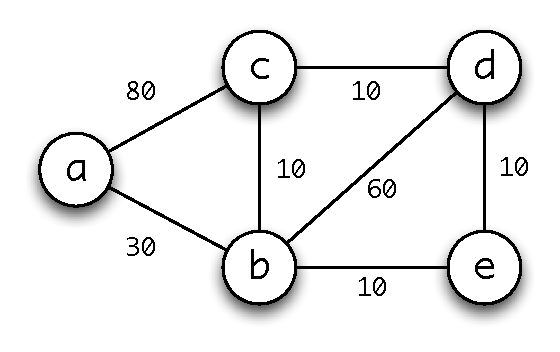
\epsfig{file=flight-costs.eps,width=0.45\columnwidth}
  \caption{Flight Map and Cost Between 5 Cities}
  \label{fig:flight}
\end{figure}

\begin{figure}[th]
\begin{lstlisting}[label=lst:tsell,caption=Ticket Seller's Agent]
enum { M = 8 };
int t[M][3] =
{{ 0,1,30 },{ 0,2,80 },{ 1,2,10 },{ 1,3,60 },
 { 1,4,10 },{ 2,1,10 },{ 2,3,10 },{ 3,4,10 }};
int main() {
  for (int i = 0; i < M; i++)
    |$\mathbf{out}$|("Ticket %d %d %d", t[i][0],t[i][1],t[i][2]);
  return 0;
}
\end{lstlisting}

\begin{lstlisting}[label=lst:tbuy,caption=Ticket Buyer's Agent]
enum { N = 5 };
void wait_for_ticket(Param p) {
  Flight &d = *((Flight *) p);
  int price;
  |$\mathbf{in}$|("Ticket %d %d &d<=%d",
      d.from, d.next, &price, d.cash);
  fly(d.next, d.to, d.cash - price);
  |$\mathbf{cm}$|();
}
void fly(int from, int to, int cash) {
  Flight    flt[N];
  Function  choices[N];
  Param     params[N];
  if (from == to) return;
  set_visited(from);
  vector<int> next = unvisited_neighbors();
  for (int i = 0; i < next.size(); i++) {
    flt[i] = Flight(from, next[i], to, cash);
    choices[i] = wait_for_ticket;
    params[i] = (Param)&(flt[i]);
  }
  |$\mathbf{speculate}$|(choices, params, next.size());
}
int main() { fly(0, N-1, 100); return 0; }
\end{lstlisting}
\end{figure}

\subsection{Evaluation Results}

%\RY{just say Intel XYZ with info from /proc/cpuinfo)}
We evaluate our runtime system running these benchmarks
on Ubuntu Linux (3.2.0) with an Intel 2-core 2.7GHz CPU and 2GB RAM.
Benchmark programs are written in C++ and compiled using \texttt{g++} (4.6.3).

\begin{figure*}[th]
\centering
% DP
\subfigure[DP: Max Memory Consumption]{
  \label{fig:dp-mem}
  \epsfig{file=dp-mem.eps,width=0.24\textwidth}}
\subfigure[DP: Max \# of Concur. Worlds]{
  \label{fig:dp-world}
  \epsfig{file=dp-world.eps,width=0.24\textwidth}}
\subfigure[DP: Total CPU Time]{
  \label{fig:dp-cpu}
  \epsfig{file=dp-cpu.eps,width=0.24\textwidth}}
\subfigure[DP: \% Time Saving Due to Exit]{
  \label{fig:dp-exit}
  \epsfig{file=dp-exit.eps,width=0.24\textwidth}}
% BJ
\subfigure[BJ: Max Memory Consumption]{
  \label{fig:bj-mem}
  \epsfig{file=bj-mem.eps,width=0.24\textwidth}}
\subfigure[BJ: Max \# of Concur. Worlds]{
  \label{fig:bj-world}
  \epsfig{file=bj-world.eps,width=0.24\textwidth}}
\subfigure[BJ: Total CPU Time]{
  \label{fig:bj-cpu}
  \epsfig{file=bj-cpu.eps,width=0.24\textwidth}}
\subfigure[BJ: \% Time Saving Due to Exit]{
  \label{fig:bj-exit}
  \epsfig{file=bj-exit.eps,width=0.24\textwidth}}
% FR
\subfigure[FR: Max Memory Consumption]{
  \label{fig:fr-mem}
  \epsfig{file=fr-mem.eps,width=0.24\textwidth}}
\subfigure[FR: Max \# of Concur. Worlds]{
  \label{fig:fr-world}
  \epsfig{file=fr-world.eps,width=0.24\textwidth}}
\subfigure[FR: Total CPU Time]{
  \label{fig:fr-cpu}
  \epsfig{file=fr-cpu.eps,width=0.24\textwidth}}
\subfigure[FR: \% Time Saving Due to Exit]{
  \label{fig:fr-exit}
  \epsfig{file=fr-exit.eps,width=0.24\textwidth}}
%
\caption{Evaluation Results}
\label{fig:eval}
\end{figure*}
In each benchmark, we conducted four experiments: with 10, 20, 30 and 40
concurrent agents. In the case of BJ, this means 5, 10, 15 and 20 pairs of 
Bob/Jill programs. We ran each experiment 5 times and record the average and
maximum values for three key metrics: 
maximum memory consumption, maximum number of simultaneous worlds and 
total CPU time. 
In addition, we record the percentage time savings of each agent by
\begin{equation*}
\frac{\rm{exit\ time\ of\ last\ agent\ in\ system} - 
\rm{exit\ time\ of\ this\ agent}}
{\rm{exit\ time\ of\ last\ agent\ in\ system}}
\end{equation*}
because without exit mechanism in the system, all agents would have waited
till the last agent completes to exit from the system together. 

Figure \ref{fig:eval} shows the results.
We can see that even though theoretically the
maximum number of worlds in these examples are prohibitively large 
(i.e., $2^n$),
in reality, with the help of the commit operators, we can keep
the size of the universe as well as other computation costs
down to very manageable. In other words, given well programed agents and a
reasonable commit mechanism, the prototype system can manage 
the exponentiality inherent in the problems while achieving 
solutions for all agents in reasonable time. 

Furthermore, Figure \ref{fig:dp-exit}, \ref{fig:bj-exit} and 
\ref{fig:fr-exit} show the distributions of agents on the time savings due to
the exit semantics. Most of the agents save at least half of the overall time
with the exit semantics implemented. DP has slightly less savings in time because
most of the worlds do have solutions and hence all agents come and leave very quickly
and thus keeps the universe very small, which is evident from Figures
\ref{fig:dp-world} and \ref{fig:dp-cpu}.
Overall, the results clearly demonstrate
that the exit mechanism significantly improves the user responsiveness and 
the efficiency of the computation.
Our prototype is general in the sense that it
works with arbitrary C/C++ agents. A carefully engineered
application which uses the speculative nondeterminism model
should be even more efficient.
